%%%%%%%%%%%%%%%%%%%%%%%%%%%%%%%%%%%%%%%%%%%%%%%%%%%%%%%%%%%%%%%%%%%%%%%%%%%%%%%%
%
% Template license:
% CC BY-NC-SA 3.0 (http://creativecommons.org/licenses/by-nc-sa/3.0/)
%
%%%%%%%%%%%%%%%%%%%%%%%%%%%%%%%%%%%%%%%%%%%%%%%%%%%%%%%%%%%%%%%%%%%%%%%%%%%%%%%%

%----------------------------------------------------------------------------------------
%	PACKAGES AND OTHER DOCUMENT CONFIGURATIONS
%----------------------------------------------------------------------------------------
\documentclass[
11pt, % The default document font size, options: 10pt, 11pt, 12pt
%oneside, % Two side (alternating margins) for binding by default, uncomment to switch to one side
%chapterinoneline,% Have the chapter title next to the number in one single line
spanish,
singlespacing, % Single line spacing, alternatives: onehalfspacing or doublespacing
%draft, % Uncomment to enable draft mode (no pictures, no links, overfull hboxes indicated)
%nolistspacing, % If the document is onehalfspacing or doublespacing, uncomment this to set spacing in lists to single
%liststotoc, % Uncomment to add the list of figures/tables/etc to the table of contents
%toctotoc, % Uncomment to add the main table of contents to the table of contents
parskip, % Uncomment to add space between paragraphs
%codirector, % Uncomment to add a codirector to the title page
headsepline, % Uncomment to get a line under the header
]{MastersDoctoralThesis} % The class file specifying the document structure
\usepackage{graphicx}
\usepackage{makecell}



%----------------------------------------------------------------------------------------
%	INFORMACIÓN DE LA MEMORIA
%----------------------------------------------------------------------------------------

\thesistitle{Sistema de monitoreo de consumo eléctrico} % El títulos de la memoria, se usa en la carátula y se puede usar el cualquier lugar del documento con el comando \ttitle

% Nombre del posgrado, se usa en la carátula y se puede usar el cualquier lugar del documento con el comando \degreename
\posgrado{Carrera de Especialización en Internet de las Cosas} 
\author{Ing. Matías Herreros} % Tu nombre, se usa en la carátula y se puede usar el cualquier lugar del documento con el comando \authorname

\director{Esp. Ing. Hernán San Martin (UNDEF - FIE)} % El nombre del director, se usa en la carátula y se puede usar el cualquier lugar del documento con el comando \dirname
\codirector{Nombre del codirector (pertenencia)} % El nombre del codirector si lo hubiera, se usa en la carátula y se puede usar el cualquier lugar del documento con el comando \codirname.  Para activar este campo se debe descomentar la opción "codirector" en el comando \documentclass, línea 23.

\juradoUNO{Nombre del jurado 1 (pertenencia)} % Nombre y pertenencia del un jurado se usa en la carátula y se puede usar el cualquier lugar del documento con el comando \jur1name
\juradoDOS{Nombre del jurado 2 (pertenencia)} % Nombre y pertenencia del un jurado se usa en la carátula y se puede usar el cualquier lugar del documento con el comando \jur2name
\juradoTRES{Nombre del jurado 3 (pertenencia)} % Nombre y pertenencia del un jurado se usa en la carátula y se puede usar el cualquier lugar del documento con el comando \jur3name

\ciudad{ciudad de Campana (Buenos Aires)}

\fechaINICIO{febrero de 2024}
\fechaFINAL{diciembre de 2024}


\keywords{Internet de las cosas, FIUBA} % Keywords for your thesis, print it elsewhere with \keywordnames


\begin{document}


\frontmatter % Use roman page numbering style (i, ii, iii, iv...) for the pre-content pages

\pagestyle{plain} % Default to the plain heading style until the thesis style is called for the body content


%----------------------------------------------------------------------------------------
%	RESUMEN - ABSTRACT 
%----------------------------------------------------------------------------------------

\begin{abstract}
\addchaptertocentry{\abstractname} % Add the abstract to the table of contents
%
%The Thesis Abstract is written here (and usually kept to just this page). The page is kept centered vertically so can expand into the blank space above the title too\ldots
\centering
La presente memoria describe el diseño y la implementación del prototipo de un dispositivo que permite medir distintas variables relacionadas al consumo eléctrico. Este sistema transmite los datos recolectados a un servidor en la nube donde son procesados, almacenados y puestos a disposición a través de una plataforma web. A partir de la información obtenida los usuarios pueden, de una forma práctica, monitorear su consumo.

La memoria incluye detalles sobre la arquitectura del sistema, su implementación y pruebas realizadas, así como los resultados obtenidos. A lo largo del desarrollo del trabajo se aplicaron conocimientos relacionados con el diseño de hardware, desarrollo de software y administración de bases de datos.

\end{abstract}

%----------------------------------------------------------------------------------------
%	CONTENIDO DE LA MEMORIA  - AGRADECIMIENTOS
%----------------------------------------------------------------------------------------

%\begin{acknowledgements}
%\addchaptertocentry{\acknowledgementname} % Descomentando esta línea se puede agregar los agradecimientos al índice
%\vspace{1.5cm}

%Esta sección es para agradecimientos personales y es totalmente \textbf{OPCIONAL}.  

%\end{acknowledgements}

%----------------------------------------------------------------------------------------
%	LISTA DE CONTENIDOS/FIGURAS/TABLAS
%----------------------------------------------------------------------------------------

\tableofcontents % Prints the main table of contents

\listoffigures % Prints the list of figures

\listoftables % Prints the list of tables


%----------------------------------------------------------------------------------------
%	CONTENIDO DE LA MEMORIA  - DEDICATORIA
%----------------------------------------------------------------------------------------

%\dedicatory{\textbf{Dedicado a... [OPCIONAL]}}  % escribir acá si se desea una dedicatoria

%----------------------------------------------------------------------------------------
%	CONTENIDO DE LA MEMORIA  - CAPÍTULOS
%----------------------------------------------------------------------------------------

\mainmatter % Begin numeric (1,2,3...) page numbering

\pagestyle{thesis} % Return the page headers back to the "thesis" style

% Incluir los capítulos como archivos separados desde la carpeta Chapters


% Chapter 1

\chapter{Introducción general} % Main chapter title
En el presente capítulo se presenta una descripción del contexto y la importancia de contar con información precisa sobre el consumo energético. Además, se aborda la motivación detrás del trabajo, subrayando la necesidad de reducir el impacto ambiental y los costos asociados al consumo eléctrico, se presentan los objetivos y el alcance y se detallan las metas específicas. Finalmente, se realiza una análisis sobre el estado del arte de las tecnologías relacionadas existentes en la actualidad.

\label{Chapter1} % For referencing the chapter elsewhere, use \ref{Chapter1} 
\label{IntroGeneral}


%----------------------------------------------------------------------------------------

% Define some commands to keep the formatting separated from the content 
\newcommand{\keyword}[1]{\textbf{#1}}
\newcommand{\tabhead}[1]{\textbf{#1}}
\newcommand{\code}[1]{\texttt{#1}}
\newcommand{\file}[1]{\texttt{\bfseries#1}}
\newcommand{\option}[1]{\texttt{\itshape#1}}
\newcommand{\grados}{$^{\circ}$}

%----------------------------------------------------------------------------------------

%\section{Introducción}

%----------------------------------------------------------------------------------------

\section{Sistema de monitoreo de consumo eléctrico}
Tener información es crucial para la toma de decisiones ya que mejora la calidad de las mismas al basarlas en hechos y datos concretos. Permite identificar oportunidades y riesgos, reduce incertidumbres, facilita la planificación estratégica y el uso eficiente de los recursos. 

En el ámbito de la energía, y dado el contexto actual, contar con datos de buena calidad se ha vuelto particularmente importante. En las últimas décadas, la creciente demanda de energía eléctrica ha generado preocupaciones significativas a nivel mundial. Este incremento en el consumo energético, impulsado por el crecimiento poblacional, la industrialización y la expansión de tecnologías dependientes de la electricidad, ha llevado a una mayor explotación de recursos naturales y un aumento de las emisiones de gases de efecto invernadero, como se observa en la figura \ref{fig:emisionesco2}. Estos factores han contribuido al cambio climático, provocando impactos ambientales que van desde el calentamiento global hasta la pérdida de biodiversidad y eventos climáticos extremos.

\newpage

\begin{figure}[ht]
	\centering
	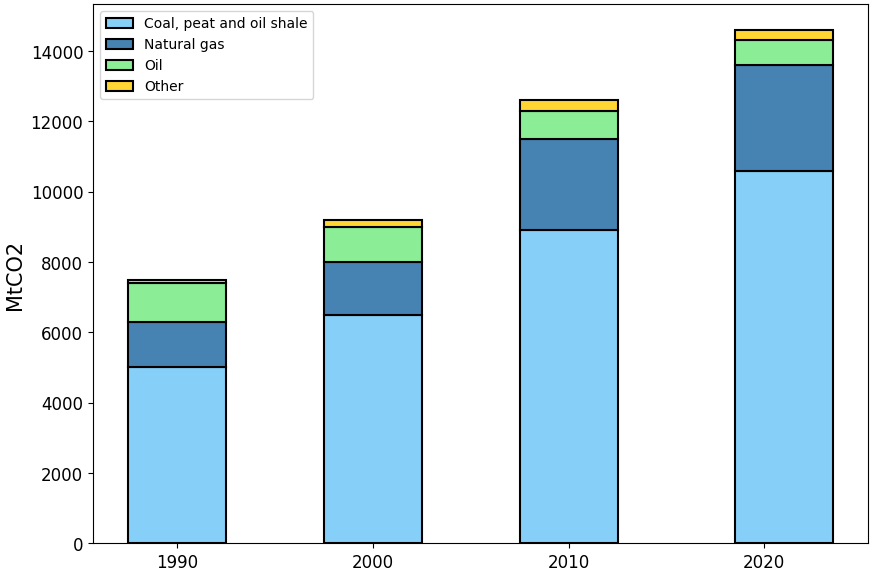
\includegraphics[width=1\textwidth]{./Figures/co2_emissions.png}
	\caption[Emisiones de $CO_2$ por la generación de electricidad.]{Emisiones de $CO_2$ por la generación de electricidad y calor por fuente de energía a nivel global\footnotemark.}
	\label{fig:emisionesco2}
	
\end{figure}

\footnotetext{IEA (2023), Greenhouse Gas Emissions from Energy Data Explorer, IEA, Paris \url{https://www.iea.org/data-and-statistics/data-tools/greenhouse-gas-emissions-from-energy-data-explorer}}

Según un informe de la \textit{International Energy Agency} (IEA) \cite{ieareport}, y como se observa en la figura \ref{fig:demandaElectricidad}, se espera que el crecimiento de la demanda global de electricidad aumente del 2,6 \% en 2023 a un promedio del 3,2 \% en 2024-2025. El estudio también destaca que para 2025, la demanda aumentará en 2500 TWh con respecto a los niveles de 2022, lo que significa que en los próximos tres años, el aumento anual del consumo de electricidad será aproximadamente equivalente a la suma del consumo de Reino Unido y Alemania juntos.

\newpage

\begin{figure}[ht]
	\centering
	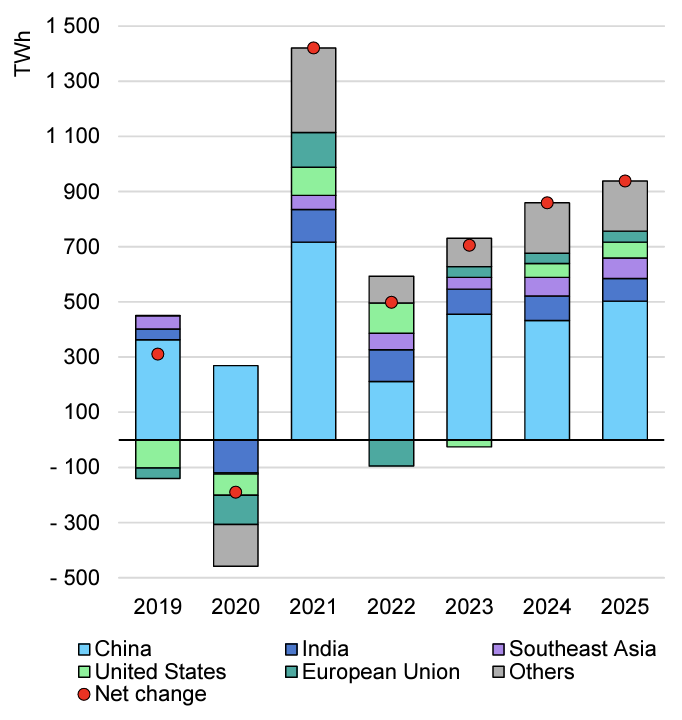
\includegraphics[width=.7\textwidth]{./Figures/year-on-year-change-in-electricity-demand-by-region-2019-2025.png}
	\caption[Cambio anual en la demanda de electricidad por región para el período 2019-2025.]{Cambio anual en la demanda de electricidad por región para el período 2019-2025\footnotemark.}
	\label{fig:demandaElectricidad}
\end{figure}

\footnotetext{IEA (2023), Year-on-year change in electricity demand by region, 2019-2025, IEA, Paris \url{https://www.iea.org/data-and-statistics/charts/year-on-year-change-in-electricity-demand-by-region-2019-2025}, Licence: CC BY 4.0}

Al mismo tiempo, el costo de la electricidad también ha experimentado un incremento significativo en los últimos años, impulsado por diversos factores como la creciente demanda, el aumento de precios de los combustibles utilizados para su generación y factores geopolíticos. Este aumento impacta directamente en el presupuesto de los hogares y en la competitividad de las industrias y la economía en general.

En este contexto, la eficiencia energética se ha convertido en una prioridad global. Gobiernos, organizaciones y consumidores buscan métodos para optimizar el uso de la energía y reducir su huella de carbono. 

Uno de los sectores donde esta optimización es crucial es el consumo eléctrico domiciliario. Los hogares representan una parte significativa del consumo energético total y, a menudo, carecen de herramientas eficaces para monitorear y gestionar su uso de electricidad. Esta falta de visibilidad y control sobre el consumo diario impide a los usuarios adoptar hábitos más sostenibles y económicos.

Para lograr una mayor eficiencia es vital poder contar con información en tiempo real relacionada al consumo de energía eléctrica. Tener estos datos permitiría, por ejemplo, identificar cuáles son los electrodomésticos y hábitos que más energía consumen o tomar decisiones informadas al reemplazar o adquirir nuevos dispositivos. Disponer de información adecuada puede ayudar a los hogares a enfocar los esfuerzos de ahorro energético, disminuir sus costos asociados y contribuir a la sostenibilidad ambiental.

\newpage
\section{Motivación}
La motivación del trabajo surge de la necesidad de abordar los desafíos previamente planteados relacionados con el consumo energético, la sostenibilidad ambiental y la economía doméstica. El sistema busca generar datos y proveer información para lograr una reducción de consumo eléctrico a partir de la adopción de prácticas más eficientes. Esta disminución y eficientización del consumo es clave ya que sirve para reducir el impacto ambiental relacionado con la generación y consumo de energía y para reducir costos.

\section{Objetivos y alcance}

\subsection{Objetivos}
El principal objetivo del trabajo es el diseño e implementación de un prototipo que permita, principalmente a usuarios domiciliarios, tener información sobre su consumo de electricidad para poder tomar decisiones inteligentes que apunten a reducir el uso de energía. El objetivo subyacente es asistir a los usuarios en la reducción de costos y generar un impacto positivo en el ambiente. Este objetivo macro se desglosa en varios objetivos específicos:

\begin{itemize}
	\item Medir variables eléctricas esenciales como tensión, corriente, potencia, frecuencia y factor de potencia.
	
	\item Asegurar que el dispositivo transmita los datos de manera confiable a un servidor en la nube para su procesamiento, almacenamiento y posterior consumo.

	\item  Proveer al usuario una interfaz intuitiva que le permita acceder a sus datos de consumo eléctrico de manera clara y comprensible.

	\item Ofrecer herramientas analíticas para identificar patrones de consumo y sugerir acciones para mejorar la eficiencia energética. 
	
	\item Fomentar el uso responsable de la energía mediante recomendaciones basadas en datos precisos.
	
	\item Educar a los usuarios sobre su consumo energético y las maneras de optimizarlo, para contribuir a la reducción de costos y del impacto ambiental.
	
	\item Asegurar que el sistema sea escalable para adaptarse a diferentes volúmenes de datos y a un número creciente de usuarios.
	
	\item Mantener la accesibilidad y facilidad de uso del sistema, para garantizar que usuarios sin conocimientos técnicos avanzados puedan beneficiarse de la herramienta.
\end{itemize}

\subsection{Alcance}

El alcance del trabajo abarca desde el diseño inicial hasta la implementación y despliegue de un sistema de monitoreo. Este sistema incluye varios componentes y fases clave de desarrollo:

\begin{itemize}
	\item Diseño y desarrollo del dispositivo de medición:
		\begin{itemize}
		\item Selección de componentes de hardware y sensores adecuados para la medición de variables eléctricas.
		\item Programación del dispositivo para la captura precisa de datos y su transmisión mediante conexión Wi-Fi.
		\end{itemize}
	\item Implementación de un servidor:
		\begin{itemize}
		\item Configuración de una base de datos relacional para el almacenamiento seguro y eficiente de grandes volúmenes de datos.
		\item Desarrollo de endpoints HTTP que permitan operaciones CRUD \cite{crud} sobre los datos y la gestión de usuarios.
		\item Implementación de un broker MQTT.
		\end{itemize}
	\item Desarrollo de la plataforma web:
	\begin{itemize}
		\item Creación de una interfaz de usuario intuitiva utilizando frameworks modernos.
		\item Integración de funcionalidades analíticas y visualización de datos, que faciliten la interpretación y el análisis del consumo eléctrico por parte de los usuarios.
	\end{itemize}
	\item Fase de pruebas y validación:
	\begin{itemize}
		\item Realización de pruebas unitarias y de integración para asegurar la correcta interacción entre el dispositivo de medición, el servidor en la nube y la plataforma web.
		\item Validación del sistema en un entorno real para garantizar su funcionalidad y eficacia.
	\end{itemize}
	\item Despliegue y mantenimiento:
	\begin{itemize}
		\item Implementación del sistema en un entorno operativo real, disponible para usuarios domésticos.
	\end{itemize}
\end{itemize} 


\newpage

\section{Estado del arte}

Existen diversas tecnologías y productos que permiten a los usuarios monitorizar y gestionar su uso de energía de manera eficiente. Estos dispositivos varían en capacidades, parámetros medidos, precios y características técnicas. 

A continuación, se presenta una comparativa de algunos de los productos más destacados en el mercado, evaluando sus capacidades, parámetros medidos, precios y especificaciones técnicas.

\begin{itemize}
    \item Sense Home Energy Monitor \cite{competencia1}: 
    Sense es una aplicación móvil que muestra cuánta energía están consumiendo el hogar y los dispositivos individuales en tiempo real. Ayuda a encontrar maneras de ahorrar dinero y reducir la huella de carbono, ofreciendo información personalizada y herramientas para rastrear los aparatos que más energía consumen.

    \item Emporia Vue \cite{competencia2}:
    el monitor de energía doméstica Emporia Vue permite monitorear el uso de energía en tiempo real e identificar cualquier consumo de energía innecesario, ayudando a ahorrar dinero. Es reconocido como el mejor monitor de energía doméstica del mercado y es líder en ventas en Amazon. Permite el monitoreo de hasta 16 circuitos individuales, con integración con asistentes de voz como Alexa para control y notificaciones.

    \item Aeotec Home Energy Meter \cite{competencia3}:
    los sensores pertenecientes a la familia Aeotec Home Energy Meter son compatibles con las tecnologías Zigbee o Z-Wave, y proporcionan datos vitales para hacer que una red doméstica sea verdaderamente inteligente. Los sensores no solo recopilan y transfieren datos, sino que también permiten activar automatizaciones vinculadas. Los datos recopilados también se utilizan para advertir, informar y proteger la instalación eléctrica en el caso que se den condiciones inusuales.

    \item TED Pro Home \cite{competencia4}:
    el T1500 es un medidor de potencia que mide con precisión el consumo de energía de los dispositivos. Tiene una funcionalidad que permite al usuario introducir el valor del kilowatt-hora (kWh) y, en base a esto, se estima el costo de la energía consumida por el electrodoméstico conectado. El T1500 también puede usarse para verificar la calidad de la energía al monitorear el tensión, la frecuencia y el factor de potencia entre otras variables. No posee forma de almacenamiento de datos históricos.

    \item Efergy Elite 4.0 \cite{competencia5}:
    este dispositivo permite ver cuánta electricidad se está usando en cualquier momento (costo y kW), ver datos promedio e históricos diarios, semanales o mensuales, configurar hasta 4 tarifas diferentes y múltiples monedas mundiales, y emitir alertas de audio frente a consumos de energía excesivos.
\end{itemize}

En la tabla \ref{tab:tablaComparativaProductos} se presenta en forma condensada la comparativa entre los distintos productos. Se consideran valores en dólares americanos (USD).

\begin{table}[h]
	\centering
        \caption[Productos actuales en el mercado]{Tabla comparativa de los productos similares presentes en el mercado.}
	\begin{tabular}{c c c c}    
		\toprule
		\textbf{Producto} 	 & \textbf{\makecell{Parámetros \\Medidos}} 		& \textbf{Precio} & \textbf{\makecell{Especificaciones \\Técnicas}}  \\
		\midrule
		\makecell{Sense Home \\Energy Monitor} & \makecell{V, A, W,\\ FP, Hz}   & \$ 300  & \makecell{Wi-Fi, detección de \\dispositivos, app móvil \\integrada, procesamiento edge.}\\	
  
		Emporia Vue	              & \makecell{V, A, W,\\ FP, Hz}   & \$ 100  & \makecell{Wi-Fi, 16 sensores de \\circuito, app móvil, \\integración con asistentes de voz.}\\
  
		\makecell{Aeotec Home \\Energy Meter}  & \makecell{V, A, W,\\ FP, Hz}   & \$ 130  & \makecell{Z-Wave, medición\\ de energía total y por fase.}\\

            TED 1500                  & \makecell{V, A, W,\\ FP, Hz}   & \$ 50   &\makecell{Pantalla LCD, batería\\ de respaldo, aviso \\de sobre tensión.}\\
            
            Efergy Elite 4.0          & \makecell{V, A, W,\\ FP, Hz}   & \$ 49   &\makecell{RF, pantalla LCD, \\almacenamiento de datos \\de hasta 24 meses.}\\
		\bottomrule
		\hline
	\end{tabular}
 	
	\label{tab:tablaComparativaProductos}
\end{table}

La selección de un sistema de monitoreo de consumo eléctrico depende de las necesidades específicas del usuario, incluyendo el nivel de detalle requerido, la facilidad de instalación y el presupuesto disponible. Los productos comparados ofrecen una gama de capacidades y características, desde la medición y visualización del consumo eléctrico en el propio dispositivo, hasta la detección avanzada de dispositivos, la integración con sistemas de domótica y la generación de informes. Esta comparativa proporciona una base para evaluar la solución presentada en el presente trabajo.


%\chapter{Introducción específica} % Main chapter title

\label{Chapter2}

%----------------------------------------------------------------------------------------
%	SECTION 1
%----------------------------------------------------------------------------------------
Todos los capítulos deben comenzar con un breve párrafo introductorio que indique cuál es el contenido que se encontrará al leerlo.  La redacción sobre el contenido de la memoria debe hacerse en presente y todo lo referido al proyecto en pasado, siempre de modo impersonal.

\section{Estilo y convenciones}
\label{sec:ejemplo}

\subsection{Uso de mayúscula inicial para los título de secciones}

Si en el texto se hace alusión a diferentes partes del trabajo referirse a ellas como capítulo, sección o subsección según corresponda. Por ejemplo: ``En el capítulo \ref{Chapter1} se explica tal cosa'', o ``En la sección \ref{sec:ejemplo} se presenta lo que sea'', o ``En la subsección \ref{subsec:ejemplo} se discute otra cosa''.

Cuando se quiere poner una lista tabulada, se hace así:

\begin{itemize}
	\item Este es el primer elemento de la lista.
	\item Este es el segundo elemento de la lista.
\end{itemize}

Notar el uso de las mayúsculas y el punto al final de cada elemento.

Si se desea poner una lista numerada el formato es este:

\begin{enumerate}
	\item Este es el primer elemento de la lista.
	\item Este es el segundo elemento de la lista.
\end{enumerate}

Notar el uso de las mayúsculas y el punto al final de cada elemento.

\subsection{Este es el título de una subsección}
\label{subsec:ejemplo}

Se recomienda no utilizar \textbf{texto en negritas} en ningún párrafo, ni tampoco texto \underline{subrayado}. En cambio sí se debe utilizar \textit{texto en itálicas} para palabras en un idioma extranjero, al menos la primera vez que aparecen en el texto. En el caso de palabras que estamos inventando se deben utilizar ``comillas'', así como también para citas textuales. Por ejemplo, un \textit{digital filter} es una especie de ``selector'' que permite separar ciertos componentes armónicos en particular.

La escritura debe ser impersonal. Por ejemplo, no utilizar ``el diseño del firmware lo hice de acuerdo con tal principio'', sino ``el firmware fue diseñado utilizando tal principio''. 

El trabajo es algo que al momento de escribir la memoria se supone que ya está concluido, entonces todo lo que se refiera a hacer el trabajo se narra en tiempo pasado, porque es algo que ya ocurrió. Por ejemplo, "se diseñó el firmware empleando la técnica de test driven development".

En cambio, la memoria es algo que está vivo cada vez que el lector la lee. Por eso transcurre siempre en tiempo presente, como por ejemplo:

``En el presente capítulo se da una visión global sobre las distintas pruebas realizadas y los resultados obtenidos. Se explica el modo en que fueron llevados a cabo los test unitarios y las pruebas del sistema''.

Se recomienda no utilizar una sección de glosario sino colocar la descripción de las abreviaturas como parte del mismo cuerpo del texto. Por ejemplo, RTOS (\textit{Real Time Operating System}, Sistema Operativo de Tiempo Real) o en caso de considerarlo apropiado mediante notas a pie de página.

Si se desea indicar alguna página web utilizar el siguiente formato de referencias bibliográficas, dónde las referencias se detallan en la sección de bibliografía de la memoria, utilizado el formato establecido por IEEE en \citep{IEEE:citation}. Por ejemplo, ``el presente trabajo se basa en la plataforma EDU-CIAA-NXP \citep{CIAA}, la cual...''.

\subsection{Figuras} 

Al insertar figuras en la memoria se deben considerar determinadas pautas. Para empezar, usar siempre tipografía claramente legible. Luego, tener claro que \textbf{es incorrecto} escribir por ejemplo esto: ``El diseño elegido es un cuadrado, como se ve en la siguiente figura:''

\begin{figure}[h]
\centering
\includegraphics[scale=.45]{./Figures/cuadradoAzul.png}
\end{figure}

La forma correcta de utilizar una figura es con referencias cruzadas, por ejemplo: ``Se eligió utilizar un cuadrado azul para el logo, como puede observarse en la figura \ref{fig:cuadradoAzul}''.

\begin{figure}[ht]
	\centering
	\includegraphics[scale=.45]{./Figures/cuadradoAzul.png}
	\caption{Ilustración del cuadrado azul que se eligió para el diseño del logo.}
	\label{fig:cuadradoAzul}
\end{figure}

El texto de las figuras debe estar siempre en español, excepto que se decida reproducir una figura original tomada de alguna referencia. En ese caso la referencia de la cual se tomó la figura debe ser indicada en el epígrafe de la figura e incluida como una nota al pie, como se ilustra en la figura \ref{fig:palabraIngles}.

\begin{figure}[htpb]
	\centering
	\includegraphics[scale=.3]{./Figures/word.jpeg}
	\caption{Imagen tomada de la página oficial del procesador\protect\footnotemark.}
	\label{fig:palabraIngles}
\end{figure}

\footnotetext{Imagen tomada de \url{https://goo.gl/images/i7C70w}}

La figura y el epígrafe deben conformar una unidad cuyo significado principal pueda ser comprendido por el lector sin necesidad de leer el cuerpo central de la memoria. Para eso es necesario que el epígrafe sea todo lo detallado que corresponda y si en la figura se utilizan abreviaturas entonces aclarar su significado en el epígrafe o en la misma figura.



\begin{figure}[ht]
	\centering
	\includegraphics[scale=.37]{./Figures/questionMark.png}
	\caption{¿Por qué de pronto aparece esta figura?}
	\label{fig:questionMark}
\end{figure}

Nunca colocar una figura en el documento antes de hacer la primera referencia a ella, como se ilustra con la figura \ref{fig:questionMark}, porque sino el lector no comprenderá por qué de pronto aparece la figura en el documento, lo que distraerá su atención.

Otra posibilidad es utilizar el entorno \textit{subfigure} para incluir más de una figura, como se puede ver en la figura \ref{fig:three graphs}. Notar que se pueden referenciar también las figuras internas individualmente de esta manera: \ref{fig:1de3}, \ref{fig:2de3} y \ref{fig:3de3}.
 
\begin{figure}[!htpb]
     \centering
     \begin{subfigure}[b]{0.3\textwidth}
         \centering
         \includegraphics[width=.65\textwidth]{./Figures/questionMark}
         \caption{Un caption.}
         \label{fig:1de3}
     \end{subfigure}
     \hfill
     \begin{subfigure}[b]{0.3\textwidth}
         \centering
         \includegraphics[width=.65\textwidth]{./Figures/questionMark}
         \caption{Otro.}
         \label{fig:2de3}
     \end{subfigure}
     \hfill
     \begin{subfigure}[b]{0.3\textwidth}
         \centering
         \includegraphics[width=.65\textwidth]{./Figures/questionMark}
         \caption{Y otro más.}
         \label{fig:3de3}
     \end{subfigure}
        \caption{Tres gráficos simples}
        \label{fig:three graphs}
\end{figure}

El código para generar las imágenes se encuentra disponible para su reutilización en el archivo \file{Chapter2.tex}.

\subsection{Tablas}

Para las tablas utilizar el mismo formato que para las figuras, sólo que el epígrafe se debe colocar arriba de la tabla, como se ilustra en la tabla \ref{tab:peces}. Observar que sólo algunas filas van con líneas visibles y notar el uso de las negritas para los encabezados.  La referencia se logra utilizando el comando \verb|\ref{<label>}| donde label debe estar definida dentro del entorno de la tabla.

\begin{verbatim}
\begin{table}[h]
	\centering
	\caption[caption corto]{caption largo más descriptivo}
	\begin{tabular}{l c c}    
		\toprule
		\textbf{Especie}     & \textbf{Tamaño} & \textbf{Valor}\\
		\midrule
		Amphiprion Ocellaris & 10 cm           & \$ 6.000 \\		
		Hepatus Blue Tang    & 15 cm           & \$ 7.000 \\
		Zebrasoma Xanthurus  & 12 cm           & \$ 6.800 \\
		\bottomrule
		\hline
	\end{tabular}
	\label{tab:peces}
\end{table}
\end{verbatim}


\begin{table}[h]
	\centering
	\caption[Comparativa de productos actuales en el mercado]{Tabla comparativa de los productos presentes en el mercado similares al desarrollado en este trabajo}
	\begin{tabular}{l c c c}    
		\toprule
		\textbf{Producto} 	 & \textbf{Parámetros Medidos} 		& \textbf{Precio} & \textbf{Especificaciones}  \\
		\midrule
		Sense Home Energy Monitor & V, A, W, FP, Hz   & \$ 300  &Wi-Fi, detección de dispositivos, \\app móvil integrada, procesamiento edge\\		
		Emporia Vue	              & V, A, W, FP, Hz   & \$ 100  &Wi-Fi, 16 sensores de circuito, \\app móvil, integración con asistentes \\de voz\\
		Aeotec Home Energy Meter  & V, A, W, FP, Hz   & \$ 130  &Z-Wave, medición de energía\\ total y por fase\\
            TED 1500                  & V, A, W, FP, Hz   & \$ 50   &Pantalla LCD, batería de\\ respaldo, aviso de sobretensión\\
            Efergy Elite 4.0          & V, A, W, FP, Hz   & \$ 49   &RF, pantalla LCD,\\ almacenamiento de datos \\de hasta 24 meses\\
		\bottomrule
		\hline
	\end{tabular}
	\label{tab:tablaComparativaProductos}
\end{table}






En cada capítulo se debe reiniciar el número de conteo de las figuras y las tablas, por ejemplo, figura 2.1 o tabla 2.1, pero no se debe reiniciar el conteo en cada sección. Por suerte la plantilla se encarga de esto por nosotros.

\subsection{Ecuaciones}
\label{sec:Ecuaciones}

Al insertar ecuaciones en la memoria dentro de un entorno \textit{equation}, éstas se numeran en forma automática  y se pueden referir al igual que como se hace con las figuras y tablas, por ejemplo ver la ecuación \ref{eq:metric}.

\begin{equation}
	\label{eq:metric}
	ds^2 = c^2 dt^2 \left( \frac{d\sigma^2}{1-k\sigma^2} + \sigma^2\left[ d\theta^2 + \sin^2\theta d\phi^2 \right] \right)
\end{equation}
                                                        
Es importante tener presente que si bien las ecuaciones pueden ser referidas por su número, también es correcto utilizar los dos puntos, como por ejemplo ``la expresión matemática que describe este comportamiento es la siguiente:''

\begin{equation}
	\label{eq:schrodinger}
	\frac{\hbar^2}{2m}\nabla^2\Psi + V(\mathbf{r})\Psi = -i\hbar \frac{\partial\Psi}{\partial t}
\end{equation}

Para generar la ecuación \ref{eq:metric} se utilizó el siguiente código:

\begin{verbatim}
\begin{equation}
	\label{eq:metric}
	ds^2 = c^2 dt^2 \left( \frac{d\sigma^2}{1-k\sigma^2} + 
	\sigma^2\left[ d\theta^2 + 
	\sin^2\theta d\phi^2 \right] \right)
\end{equation}
\end{verbatim}

Y para la ecuación \ref{eq:schrodinger}:

\begin{verbatim}
\begin{equation}
	\label{eq:schrodinger}
	\frac{\hbar^2}{2m}\nabla^2\Psi + V(\mathbf{r})\Psi = 
	-i\hbar \frac{\partial\Psi}{\partial t}
\end{equation}

\end{verbatim} 
%\include{Chapters/Chapter3}
%\include{Chapters/Chapter4} 
%\include{Chapters/Chapter5} 

%----------------------------------------------------------------------------------------
%	CONTENIDO DE LA MEMORIA  - APÉNDICES
%----------------------------------------------------------------------------------------

\appendix % indicativo para indicarle a LaTeX los siguientes "capítulos" son apéndices

% Incluir los apéndices de la memoria como archivos separadas desde la carpeta Appendices
% Descomentar las líneas a medida que se escriben los apéndices

%\include{Appendices/AppendixA}
%\include{Appendices/AppendixB}
%\include{Appendices/AppendixC}

%----------------------------------------------------------------------------------------
%	BIBLIOGRAPHY
%----------------------------------------------------------------------------------------

\Urlmuskip=0mu plus 1mu\relax
\raggedright
\printbibliography[heading=bibintoc]

%----------------------------------------------------------------------------------------

\end{document}  
